\documentclass[a4paper]{article}
\usepackage[margin = 1 in]{geometry}
\usepackage{fancyhdr}
\usepackage{lastpage}
\usepackage{ctex}
\usepackage[utf8]{inputenc} % Required for inputting international characters
\usepackage[T1]{fontenc} % Output font encoding for international characters
\usepackage[sfdefault]{ClearSans} % Use the Clear Sans font (sans serif)
\usepackage{tocloft} 
\usepackage{makecell}%导入表格宏包
\usepackage{bmpsize}
\usepackage{graphicx}
\usepackage{epstopdf}
\usepackage{caption}
\usepackage{enumitem}
\usepackage{float}
\usepackage{multirow}
\usepackage{makecell}
\usepackage{wrapfig}
\usepackage{tcolorbox}
\usepackage[hidelinks]{hyperref}
\usepackage{xcolor}

\pagestyle{fancy}
\lhead{\textsl{\href{https://team23-22.bham.team}{\textcolor{blue}{Team Contribution Report}}}}
\chead{}
\rhead{Page \thepage\ of \pageref{LastPage}}
\lfoot{}
\rfoot{}
\cfoot{}
\renewcommand{\headrulewidth}{0.4pt}
\renewcommand{\footrulewidth}{0pt}
\renewcommand{\cftsecleader}{\cftdotfill{\cftdotsep}}
\newcommand{\tabincell}[2]{\begin{tabular}{@{}#1@{}}#2\end{tabular}} %单元格内换行

\renewcommand*\contentsname{Table of Contents}

\begin{document}

%----------------------------------------------------------------------------------------
%	TITLE PAGE
%----------------------------------------------------------------------------------------

\begin{titlepage}
	
	\rule{\linewidth}{5pt}
	\raggedleft
	\fontsize{38pt}{50pt}\selectfont
    \textbf{\\Team Project\\}
    \fontsize{28pt}{60pt}\selectfont 
    for\\
    \fontsize{38pt}{60pt}\selectfont 
    \textbf{Team Contribution Report\\}
	
	\vfill % Space between the title box and author information
	
	%------------------------------------------------
	%	Author name and information
	%------------------------------------------------
	
	\parbox[t]{0.93\textwidth}{ % Box to inset this section slightly
		\raggedleft % Right align the text
		\large % Increase the font size
		{\Large By Team 23-22}\\[4pt] % Extra space after name
		Bogdan-Marian Gheorghe\_2329324\_bxg125\\
		Chance Egbon\_2194210\_cee010\\
		Gilead Bempah\_2296232\_gxb035\\
		Matthew Goulding\_2330080\_mxg183\\
		Samuel Okasia\_2345883\_sxo183\\
		Smit Navinkumar\_2327596\_sxn197\\
		Zijun Li\_2272583\_zxl183\\
	}
	
\end{titlepage}

\section*{Option Two: the team thinks contribution between members was unequal}

\textbf{active member: }
\begin{itemize}
    \item Zijun Li
    \item Gilead Bempah
    \item Samuel Okasia
\end{itemize}

{\noindent\begin{tabular}{|p{0.2\linewidth}|p{0.65\linewidth}|p{0.1\linewidth}|} 
	\hline
 \textbf{Member Name} & \textbf{Justifications of work done} & \textbf{Score}\\
 \hline
 Zijun Li & Initilize the VM, setup the CI/CD pipeline. Done whole todo list feature and GDPR policy. Created the vertical navbar and fixed some bugs of it. Add switching the theme function. Writen Latex file for every Milestone submission. Organized part of the meetings and content integration for everyone.Assist other team members to complete the feature & 22\\
 \hline
 Gilead Bempah & Developed the Anti-Procrastination feature, created the blocking Chrome Extension, assisted in the creation of the Diary, History, and Scheduler features, and helped setting up communication with the database for most features. Assisted in the development of Navbar, email and making data user-specific.& 18\\
 \hline
 Samuel Okasia & Designed and implemented login page, Designed and implemented home page, Designed and implemented History page, Tweaked Design for Anti-procrastination page, Created Logo & 16\\
 \hline
 Bogdan-Marian Gheorghe & Designed and implemented Inbox feature, Modified To-Do list Feature and Anti-procrastination feature to send emails when something specific happens like a to-do item is marked as done or when a new URL is blocked, created Gmail account and SMPT credentials for the project, linked credentials and set-up email Service along with Endpoint API. & 13\\
 \hline
 Matthew Goulding& Designed and implemented Alarm feature, Designed html for Alarm chrome extension & 11\\
 \hline
 Chance Egbon & Design and fully implemented the task I was assigned to develop, the diary feature.  This include the html, CSS and typescript of the diary feature.& 10\\
 \hline
 Smit Navinkumar& & 10\\
 \hline
\end{tabular}}

\newpage

\section*{The Outcome of the Intervention Meeting}

During the intervention meeting, our team discussed the importance of effective communication, collaboration, and active participation in the project. We acknowledged that frequent meetings and open dialogue were crucial for fostering a positive team dynamic and ensuring that every member's voice was heard.

As a result of the intervention meeting, the team members became more aware of the need for open communication and collaboration. By implementing regular meetings, we were able to allocate tasks more evenly and monitor the progress of each team member, leading to a more balanced distribution of responsibilities.

Moreover, the intervention meeting led to an increase in participation among team members. As we emphasized the value of each member's contributions, team members became more engaged and took a proactive approach to their tasks. This improved collaboration and encouraged team members to offer support and assistance when needed, resulting in a more cohesive and efficient working environment.

\section*{Justifications for unequal contributions}

Despite the intervention meeting's positive impact, some team members' engagement levels remained relatively low, particularly in terms of code updates (git commits) and task completion enthusiasm. These members did not actively participate in discussions or volunteer for tasks, leading to an imbalance in contributions. More details could check in \href{https://git.cs.bham.ac.uk/team-projects-2022-23/team23-22/-/graphs/main?ref_type=heads}{\textcolor{blue}{Contributor statistics}} and \href{https://git.cs.bham.ac.uk/team-projects-2022-23/team23-22/-/network/main?ref_type=heads}{\textcolor{blue}{Graph}}(Click for following the link)

\begin{figure}[H]
    \centering
    \begin{minipage}{0.49\textwidth}
      \centering
      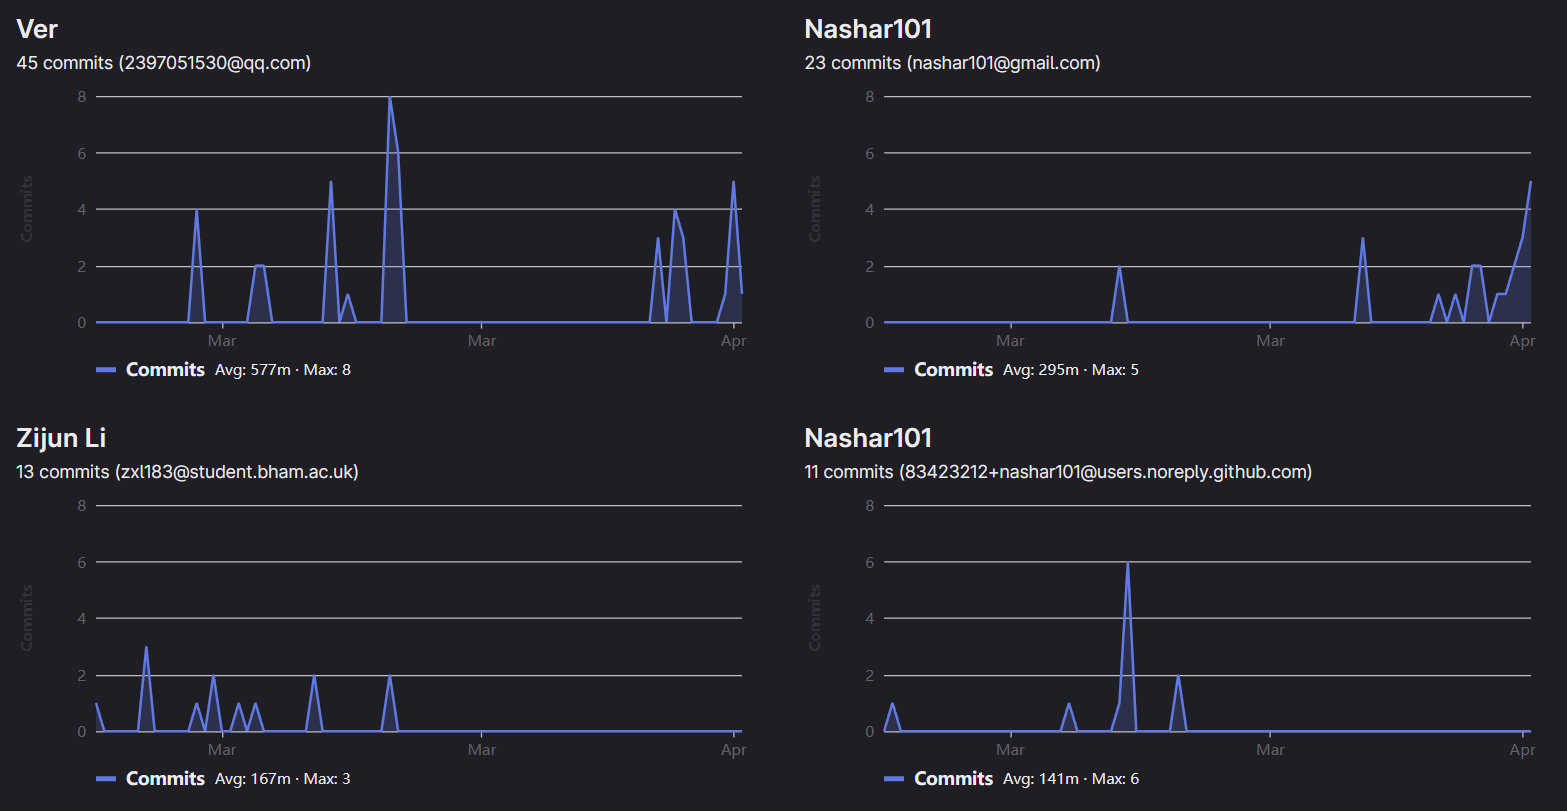
\includegraphics[width=\linewidth]{./image/Contributor_1.png}
    \end{minipage}\hfill
    \begin{minipage}{0.49\textwidth}
      \centering
      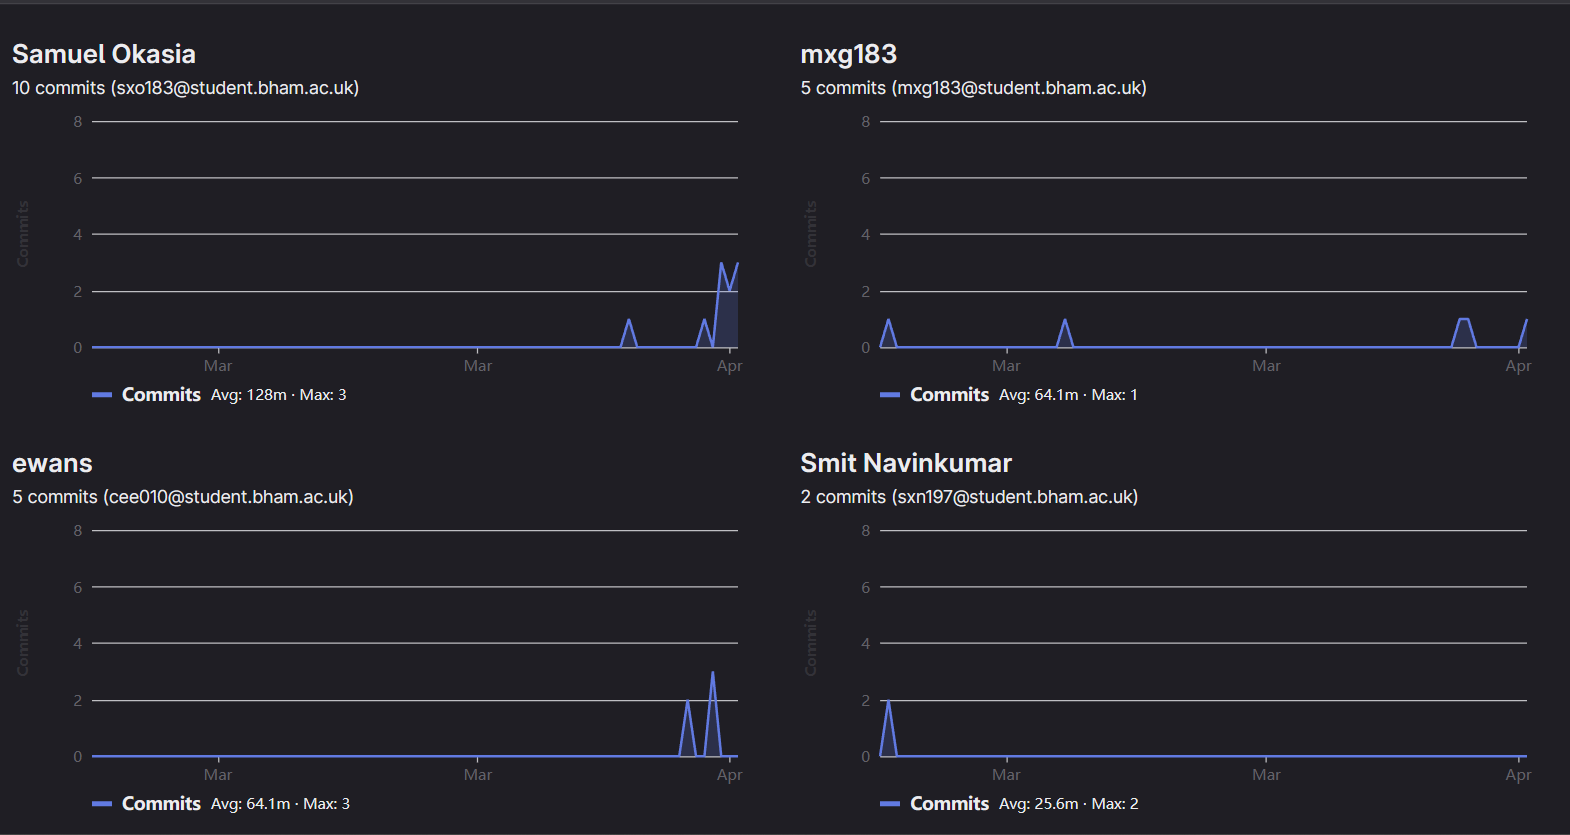
\includegraphics[width=\linewidth]{./image/Contributor_2.png}
    \end{minipage}
\end{figure}

\begin{figure}[H]
    \centering
	\begin{minipage}{0.49\textwidth}
		\centering
		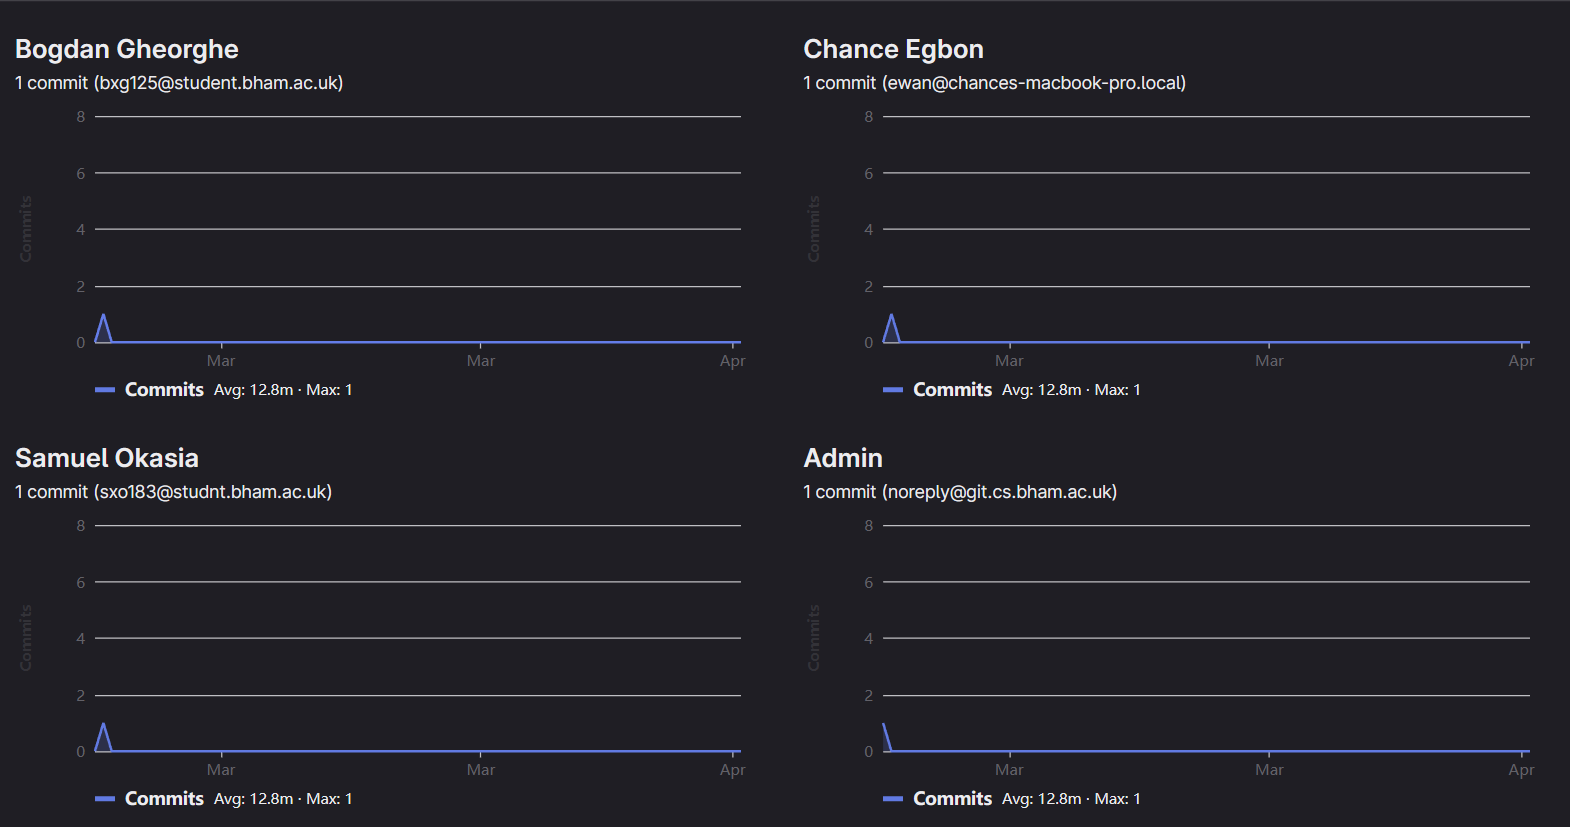
\includegraphics[width=\linewidth]{./image/Contributor_3.png}
	\end{minipage}
	\begin{minipage}{0.49\textwidth}
		\footnotesize
		Screenshot taken on 2-5-2023
		\begin{itemize}
			\item \textbf{Ver} and \textbf{Zijun} are the same person, Zijun Li
			\item Two \textbf{Nashar101} are the same person, Gilead Bempah
			\item Two \textbf{Samuel Okasia} are the same person, Samuel Okasia
			\item \textbf{mxg183} is Matthew Goulding
			\item \textbf{ewans} and  \textbf{Chance Egbon} are the same person, Chance Egbon
			\item \textbf{Smit Navinkumar} is Smit Navinkumar
			\item \textbf{Bogdan Gheorghe} is Bogdan-Marian Gheorghe
		\end{itemize}
	\end{minipage}
\end{figure}

\end{document}